\documentclass[addpoints,a4paper]{exam}

\usepackage{amsmath,amssymb,amsthm}
\usepackage[export]{adjustbox}
\usepackage{graphbox}
\usepackage{graphicx}
\usepackage{hyperref}
\usepackage{makecell}
\usepackage{tabularx}
\usepackage{titling}

\graphicspath{{images//}}

% Header and footer.
\pagestyle{headandfoot}
\runningheadrule
\runningfootrule
\runningheader{CS 412 Algorithms, Spring 2023}{Homework 2}{\theauthor}
\runningfooter{}{Page \thepage\ of \numpages}{}
\firstpageheader{}{}{}

\boxedpoints

\printanswers

\title{Homework 2\\ CS 412 Algorithms: Design and Analysis}
\author{team-name}  % replace with your team name without the brackets, e.g. q1-team-420
\date{Habib University | Spring 2023}

\begin{document}
\maketitle

\begin{questions}


  \section*{Network Flows}
  \question A group of five persons $P = \{p_1, p_2, ..., p_5\}$ plan to carpool together for each working day $d_i$ of the week. However due to several constraints (such as exams, appointments, etc.), not every person can drive on every day. The following table shows a driving possibility for each person on a given day of the week (i.e. Person $p_i$ can drive on given day $d_i$ if the corresponding element in the table is marked with an `X'):

  \begin{table}[h]
    \centering
    \renewcommand{\arraystretch}{1.5}
    \begin{tabular}{llllll}
            & Mon & Tue & Wed & Thu & Fri \\ \hline
      $p_1$ & X   & X   & X   &     &     \\ \hline
      $p_2$ & X   &     &     &     & X   \\ \hline
      $p_3$ & X   & X   &     & X   &     \\ \hline
      $p_4$ &     & X   &     & X   & X   \\ \hline
      $p_5$ &     & X   &     & X   & X   \\ \hline
    \end{tabular}%
    \caption{Table of Possibilities for each person on a given day of the week} \label{key}
  \end{table}

  A schedule is considered to be \textit{feasible} if exactly one person can be assigned one day of the week to drive.
  \begin{parts}
    \part[5] Describe an algorithm using network flows which given the above table of possibilities as an input, computes whether a it is possible to generate a feasible schedule or not ? Apply your algorithm to the above table (Table \ref{key}) to determine if it generates a feasible schedule.
    \part[5] What is the time complexity of your algorithm in terms of $n$, where the set of persons $P =  \{p_1, p_2, ..., p_n\}$ and the set of days $D = \{d_1, d_2, ..., d_n\}$ 
  \end{parts}
  \begin{solution}

  \end{solution}

  \section*{Dynamic Programming}
  \question \ \newline
  \begin{minipage}{0.2\linewidth}
    \centering
    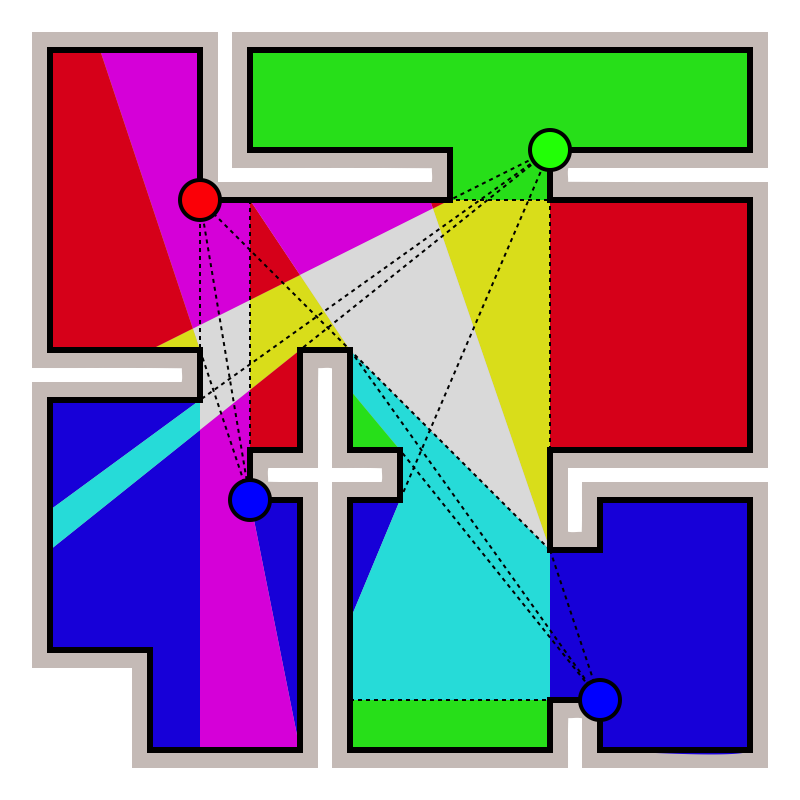
\includegraphics[width=\textwidth,align=t]{gallery}\\
    \href{https://en.wikipedia.org/wiki/Art_gallery_problem}{Wikipedia}
  \end{minipage}
  \hfill
  \begin{minipage}{0.78\linewidth}
    Consider a version of the \href{https://en.wikipedia.org/wiki/Art_gallery_problem}{art gallery problem} where the layout of the gallery is a graph, one or more artworks are placed at each node, and edges represent corridors. Placing a security camera at a node \textit{covers} the artworks at the node and its neighbors.
    \begin{parts}
      \part[5] Design a linear-time dynamic programming approach to find the minimum number of security cameras needed to cover all the artworks.
      \part[5]  Using your approach, determine the nodes at which cameras need to be placed in the gallery whose \href{https://rpruim.github.io/m252/S19/from-class/graphs/graph-representations.html}{edge list representation} is: $\{[n_1,n_2], [n_1, n_3], [n_2,n_4], [n_2, n_5],[n_3,n_6], [n_5, n_7],[n_5,n_8]\}$.
    \end{parts}
  \end{minipage}

  \begin{solution}

  \end{solution}

  \question \ \newline
  \begin{minipage}[m]{0.25\linewidth}
    \centering
    \ \newline
    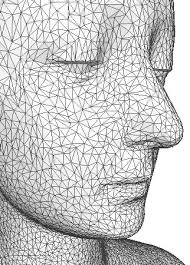
\includegraphics[width=.8\textwidth,valign=t]{mesh}\\
    \href{http://glasnost.itcarlow.ie/~powerk/GeneralGraphicsNotes/meshes/polygon_meshes_old.html}{\small 3D Object Representations}
  \end{minipage}
  \hfill
  \begin{minipage}[t]{0.73\linewidth}
    \begin{tabularx}{\textwidth}{Xc}
      Modern rendering hardware is optimized for triangles. Any 3D object to be rendered has to be \textit{triangulated}, because of which the \textit{triangle mesh} is the de-facto choice of representation for 3D objects. It is known that any polygon can be triangulated, however the triangulations are not generally unique.
       &
      \makecell[t]{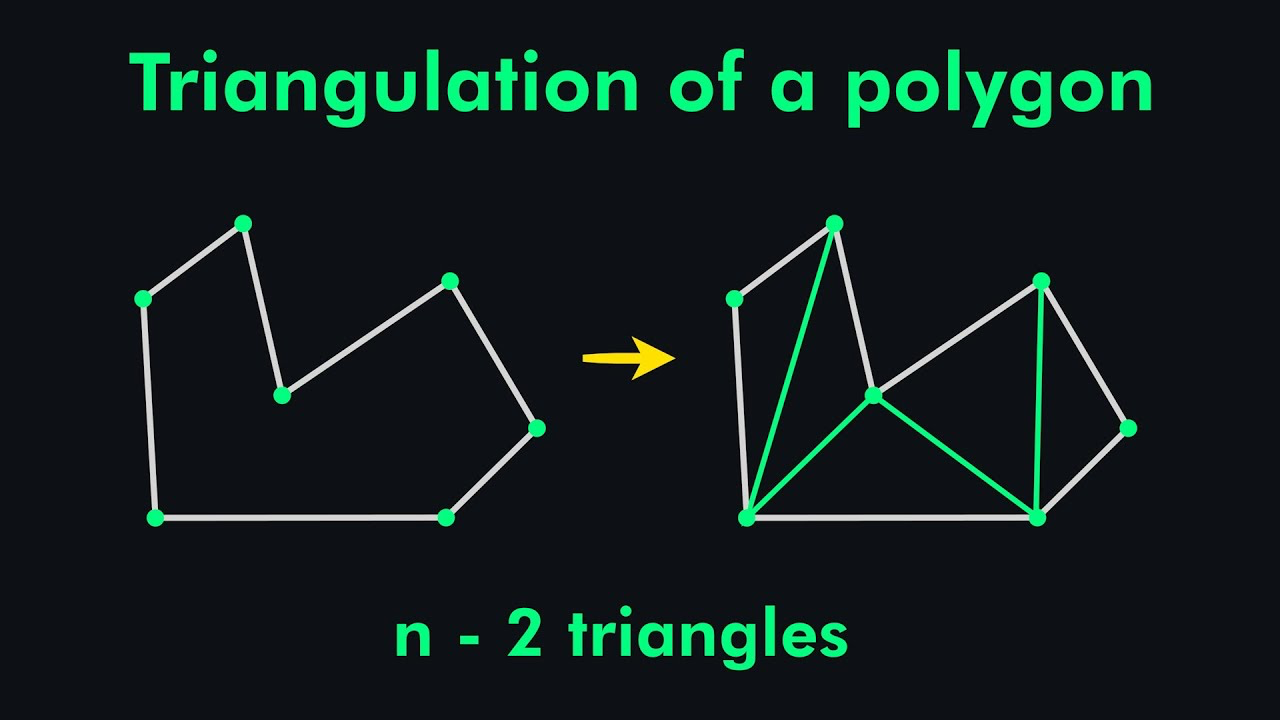
\includegraphics[width=.35\textwidth,valign=t]{triangulate} \\
        \href{https://www.youtube.com/watch?v=2x4ioToqe_c}{YouTube}}
    \end{tabularx}
    \begin{parts}
      \part[5] Devise a dynamic programming approach to compute the number of triangulations of a polygon with $n$ vertices.
      \part[5] Argue about the complexity of your approach.
    \end{parts}
  \end{minipage}

  \begin{solution}

  \end{solution}

  \section*{Greedy Algorithms}

  \question
  The \textit{coin change} problem is as follows.

  \begin{quote}

    \underline{Input}:
    \begin{itemize}
      \item A non-empty set of positive coin denominations $d_1, d_2, \ldots, d_n$.
      \item A positive integer $m$.
    \end{itemize}
    \underline{Output}: The minimum number of coins required to make change for $m$.
  \end{quote}
  Mathematically, we want to minimize the total number of coins $\sum c_i$ such that $\sum c_i d_i = m$.
  \begin{parts}
    \part[5] Given coin denominations, $1,2,4,8,\ldots,2^k$, and a positive amount, $m<2^{k+1}$, provide an $O(\lg m)$-time algorithm to find the minimum number of coins required to make change for $m$. Justify the correctness and complexity of your algorithm.
    \part[5] Provide a set of denominations for which you can prove that the greedy approach correctly finds the minimum number of coins required to make change. Also provide the proof.
    \part[5] Compare and contrast this problem with the knapsack problem.
  \end{parts}

  \begin{solution}

  \end{solution}

\end{questions}

\end{document}

%%% Local Variables:
%%% mode: latex
%%% TeX-master: t
%%% End:
